\documentclass[11pt, a4paper]{article}
\usepackage[a4paper, margin=2.5cm]{geometry}
\usepackage[english, bidi=basic, provide=*]{babel}
\babelprovide[import, onchar=ids fonts]{english}
\usepackage{booktabs}
\usepackage{tabularx}
\usepackage{graphicx}
\usepackage[table]{xcolor}
\usepackage{hyperref}

\renewcommand{\familydefault}{\sfdefault}

\definecolor{primary}{RGB}{180, 20, 30}
\definecolor{textdark}{RGB}{35, 40, 48}
\definecolor{muted}{RGB}{100, 110, 120}
\definecolor{rowtint}{RGB}{248, 249, 250}

\hypersetup{
	colorlinks=true,
	linkcolor=primary,
	urlcolor=primary
}

\setlength{\parindent}{0pt}
\setlength{\parskip}{0.6em}

\begin{document}
	
	% --- TITLE & METADATA HEADER ---
	{\color{primary}\rule{\linewidth}{2pt}}\vspace{0.6em}
	{\LARGE\bfseries\color{textdark} DHBW Compass App}\\[0.3em]
	{\large\color{muted} Project Inception Document} \\
	\vspace{0.3em}
	{\color{primary}\rule{\linewidth}{0.8pt}}
	
	\vspace{0.8em}
	
	\begin{tabularx}{\linewidth}{@{} l X r X @{}}
		\textbf{Author:} & Team 8 & \textbf{Date:} & 20 November 2026 \\
	\end{tabularx}
	
	\vspace{1em}
	
	\section{Problem Statement \& Motivation}
	
	\subsection{Problem Statement}
	Students lack a single source for planning and tracking their studies.
	Module handbooks are long and hard to read, so it is difficult to get an overview of modules, exams, and their weighting. Dualis only shows past and current grades. It offers no view of upcoming modules and no way to estimate the final grade. Valuable knowledge from older students, such as how hard a module really is, how much work it takes, and what the exam is like, gets lost or is passed on only informally. As a result, students often misjudge their workload and prepare for exams with incomplete information.
	
	\subsection{Motivation}
	The app gives students an overview of all modules, exams, and grades in one place. The module plan only needs to be set up once per course of study and could then be used by everyone in that program. Reviews, exam tips, and difficulty ratings from older classes help younger students estimate the real effort a module takes. An integrated grade calculator lets students combine their actual grades with estimated grades for upcoming exams to calculate their theoretical overall average. It also works the other way around: students can see which results they need in upcoming exams to reach their target average. This helps students plan realistically and prepare better.
	
	\section{Proposed Solution}
	\subsection{Overview}
	The proposed solution is a student companion app designed to provide useful information for academic planning. By combining peer-sourced insights with an academic tracking tool, the platform pairs official module catalogs with sharing experience between younger and experienced students.
	
	\clearpage
	\subsection{Core features}

		\textbf{Account Setup}
		
		Register, log in, and initialize a personalized module plan by selecting an existing program or uploading and analyzing the official module handbook.
		
		\textbf{Module Overview}
		
		View all required and elective modules, including associated exam types, credit points (ECTS), and grade weightings.
		
		\textbf{Peer Reviews}
		
		Read and submit difficulty/workload ratings, experience reports, and exam tips from/for fellow students.
		
		\textbf{Grade Tracking \& Simulator} 
		
		Enter achieved grades to track academic progress, simulate expected grades of upcoming exams to calculate the scores required to reach a target GPA.
	
	\subsection{Scope boundaries}
		\begin{tabularx}{\linewidth}{@{} X | X @{}}
		\textbf{In scope} & \textbf{Out of scope} \\
		\toprule
		Module browsing, submitting and viewing peer reviews, exam tip sharing
		&
		Hosting copyrighted lecture materials or past exam papers (Moodle)
		\\
		\midrule
		Personal grade tracking and GPA simulation
		&
		Official university enrollment or exam registration, direct integration with university databases (Dualis)
	\end{tabularx}
	
\section{User Groups}
	
	\textbf{Current students}
	
	Use the app to explore study modules, read student experiences and exam tips, and review difficulty ratings. They can also use the grade simulator to track their academic progress and plan possible exam results.
	
	\textbf{First-year students}
	 
	Use the app to get an overview of study modules and their expected workload. Experiences and tips from more advanced students can help them plan their studies.
	
	\textbf{Advanced students}
	
	Use the app to find information about modules and exams and to plan their academic progress. They can also share their experiences, exam tips, and assessments with other students.
	
	\textbf{Former students and alumni}
	 
	Can share their past experiences and exam tips to help current students assess the modules.
	
\section{Stakeholders}
	
	\textbf{Students and the student representative body}
	 
	Have an interest in the app providing useful, clear information about modules and exams. The student representative body can communicate students’ needs and concerns.
	
	\textbf{The university and program management}
	
	Have an interest in the app supporting the organization of studies and presenting information about study modules appropriately.
	
	\textbf{Lecturers and module coordinators}
	
	Are affected by the published experiences, exam tips, and difficulty ratings. They have an interest in content being presented fairly and objectively.
	
	\section{Use cases}
	Figure \ref{fig:usecase} shows the proposed use cases.
	
	\begin{figure}[htbp]
		\centering
		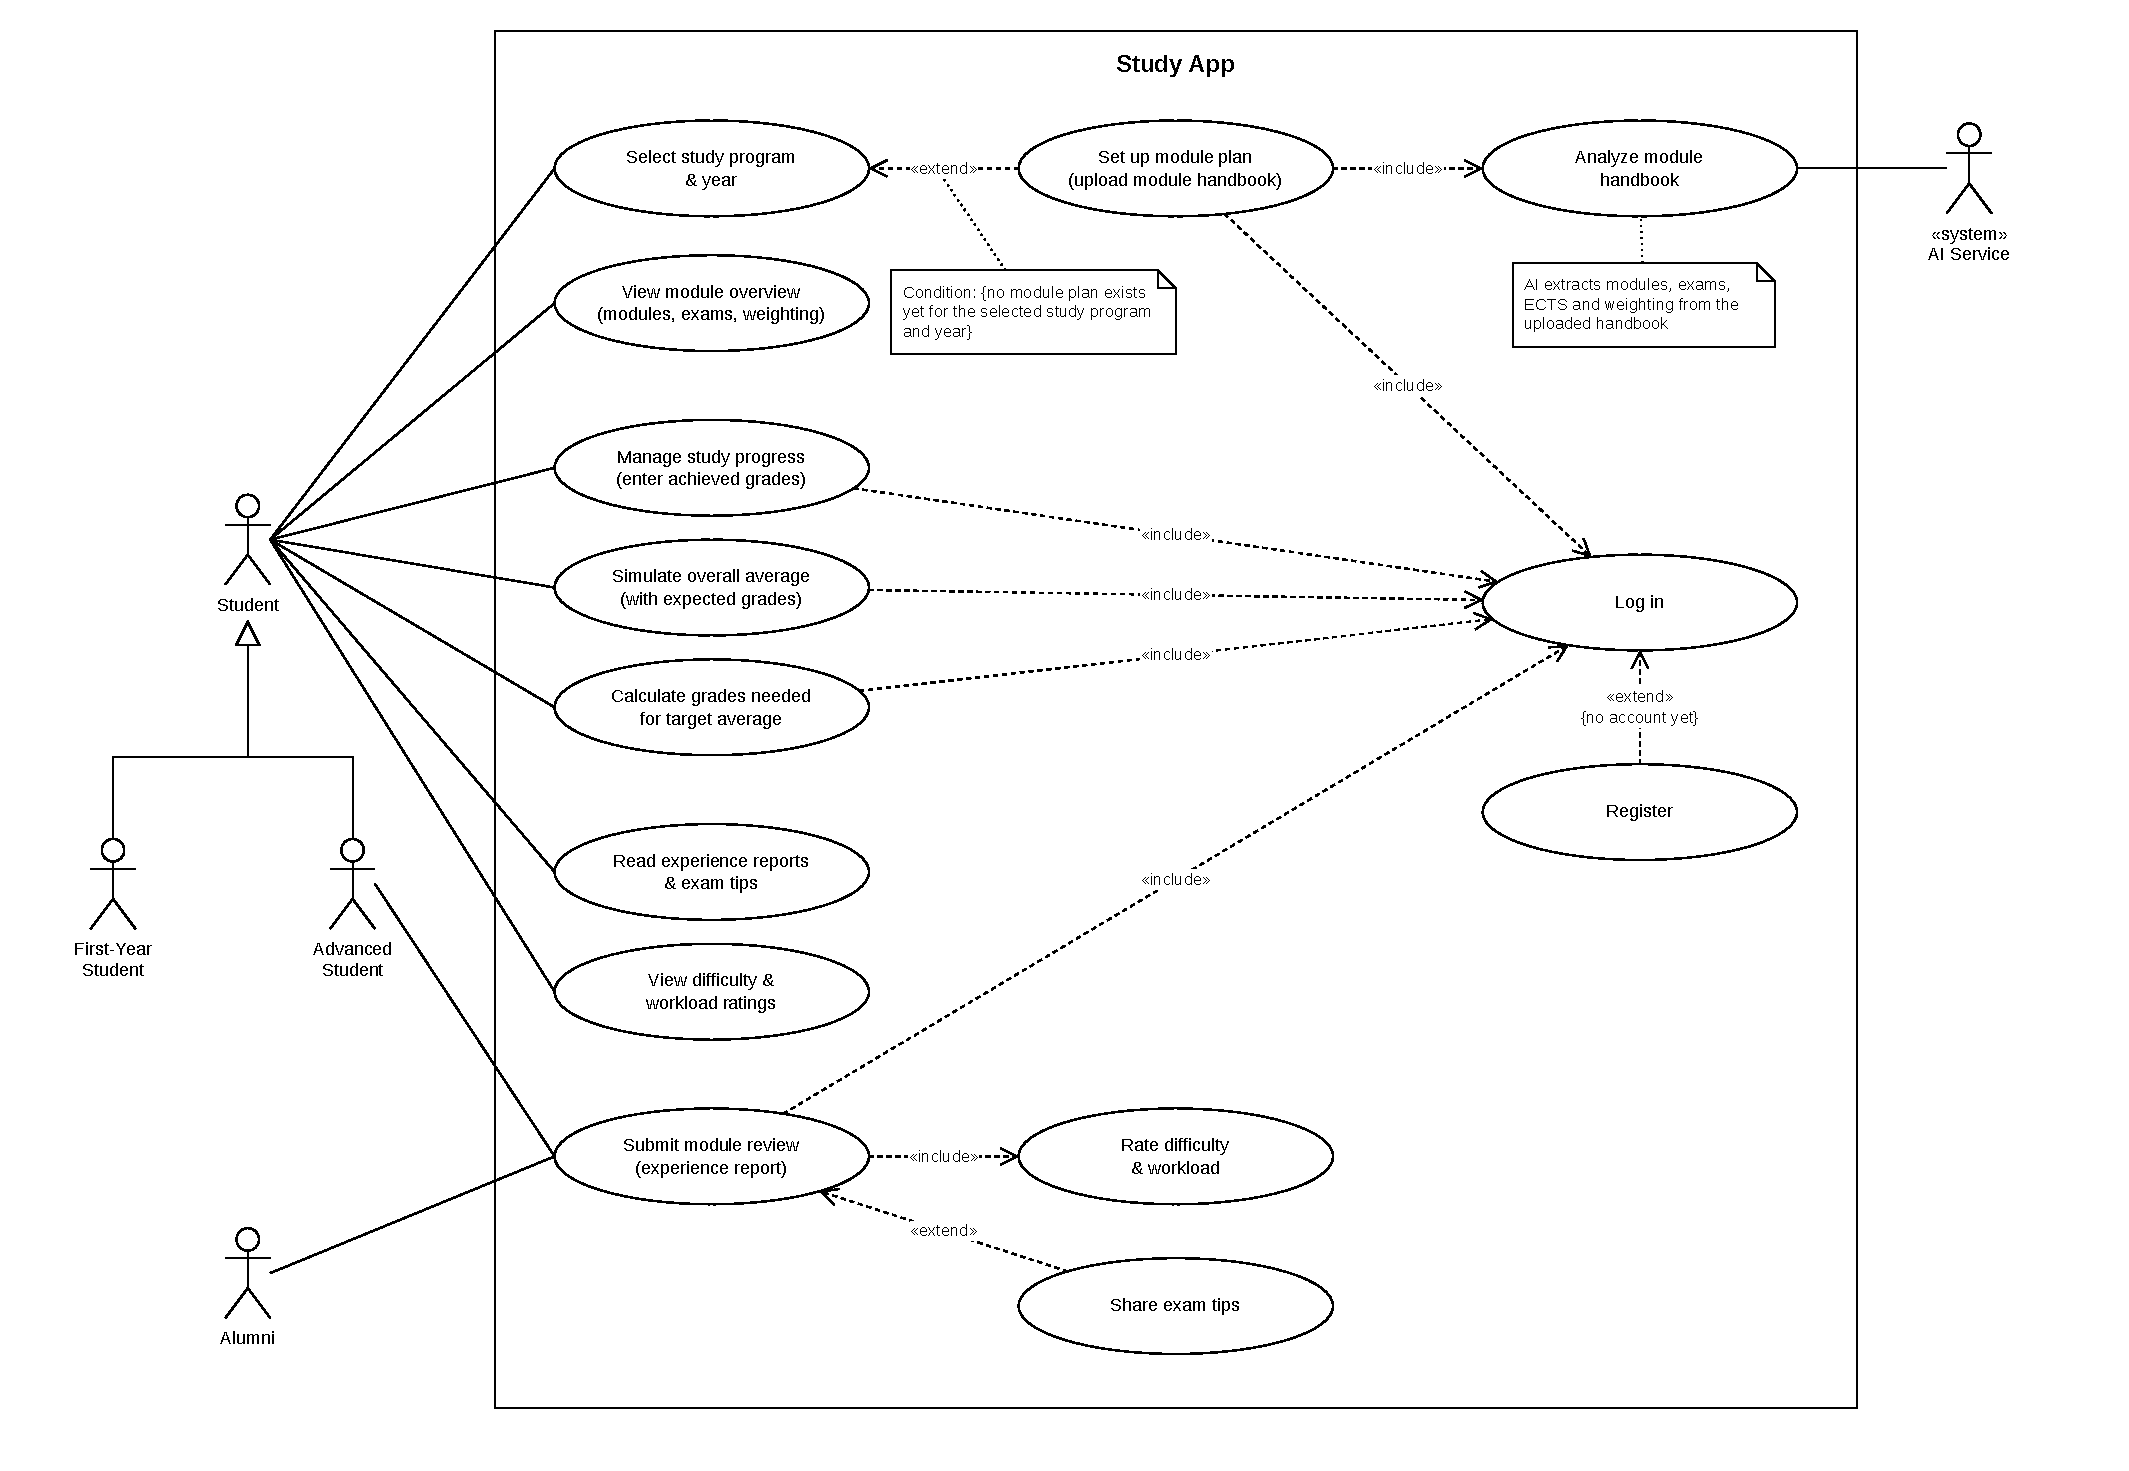
\includegraphics[width=1\textwidth]{include/usecase1}
		\caption{Initial use case diagram}
		\label{fig:usecase}
	\end{figure}
	
\end{document}